\chapter{Segmentation}

To select a certain type of tissue from an image it's used the segmentation feature at InVesalius.

\section{Threshold}

Limiar é uma técnica de segmentação de imagens que permite selecionar da imagem somente os \textit{pixels} cuja intensidade está dentro de um limiar definido pelo usuário.  O limiar é definido por dois números, limiares inicial e final, também conhecidos como \textit{thresholds} mínimo e máximo. Como referência para a definição, é utilizada a escala de Hounsfield (tabela \ref{tab:escala_hounsfield}).

In thresholding segmentation technique only the \textit{pixels} whose intensity is inside threshold range defined by the user. Threshold is defined by two number, the initial and final threshold, also known as minimum and maximum threshold. ...

Thresholding segmentation is located at the InVesalius left-panel, item \textbf{2. Select region of interest} (figure~\ref{fig:region_selection}).

\begin{figure}[!htb]
\centering
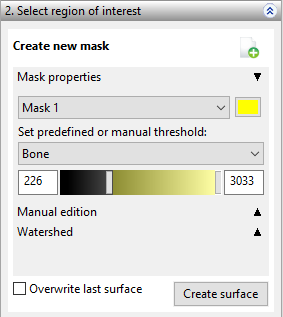
\includegraphics[scale=0.7]{segmentation_threshold_window_left_en.png}
\caption{Select region of interest - Threshold}
\label{fig:region_selection}
\end{figure}

Before starting segment it's necessary to configure a mask. A mask is a image overlayed to exam image where the selected regions are colored. See figure~\ref{fig:region_selection_masc}

\begin{figure}[!htb]
\centering
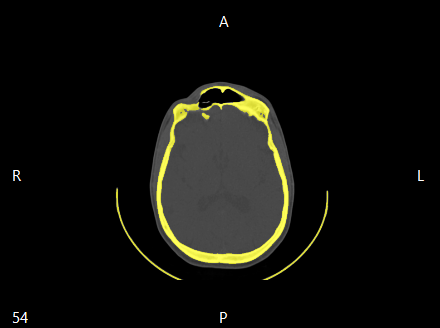
\includegraphics[scale=0.4]{segmentation_threshold_axial_en.png}
\caption{Mask - selected region in yellow.}
\label{fig:region_selection_masc}
\end{figure}

To change the threshold you may use the control that represents the image grayscale (figure~\ref{fig:region_selection_bar}). Move the \textit{left} sliding control to change the initial threshold. Move the \textit{right} sliding control to change the final threshold. It's also possible to to digit the desired threshold values in the text boxes in the left and right side of the thresholding control. Changing the thresholding values, automatically the mask will be updated, showing with a color the \textit{pixel} that are inside the thresholding range.


\begin{figure}[!htb]
\centering
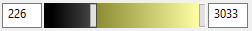
\includegraphics[scale=0.75]{segmentation_threshold_bar.png}
\caption{Selecting the \textit{pixels} with intensity between $226$ and $3021$ (Bone)}
\label{fig:region_selection_bar}
\end{figure}

It's also possible to select some predefined thresholding values based on some type of tissues, like displayed in the figure~\ref{fig:limiar_presets}. Just select the desired tissue and the mask automatically updated.

\begin{figure}[!htb]
\centering
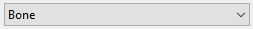
\includegraphics[scale=0.65]{segmentation_threshold_presets_en.png}
\caption{Selection list with some predefined thresholding values.}
\label{fig:limiar_presets}
\end{figure}

The table~\ref{tab:limiar} show thresholding values according to some tissues or materials.

\begin{table}[h]
\centering
\caption{Predefined thresholding values to some materials}
\begin{tabular}{lcc}\\
\hline % este comando coloca uma linha na tabela
Material & Initial threshold & Final Threshold\\
\hline
\hline
Bone & 226 & 3021\\
Compact Bone (Adult) & 662 & 1988\\
Compact Bone (Child) & 586 & 2198\\
Custom & User Def. & User Def.\\
Enamel (Adult) & 1553 & 2850\\
Enamel (Child) & 2042 & 3021\\
Fat Tissue (Adult) & -205 & -51\\
Fat Tissue (Child) & -212 & -72\\
Muscle Tissue (Adult) & -5 & 135\\
Muscle Tissue (Child) & -25 & 139\\
Skin Tissue (Adult) & -718 & -177\\
Skin Tissue (Child) & -766 & -202\\
Soft Tissue & -700 & 225\\
Spongial Bone (Adult) & 148 & 661\\
Spongial Bone (Child) & 156 & 585\\
\hline
\end{tabular}
\label{tab:limiar}
\end{table}
\newpage

The table~\ref{tab:limiar} is indicated to images obtained from medical tomographs. The range of gray values from images obtained from odontological tomographs are greater and non-regular. Thus, it's necessary to use sliding control (figure~\ref{fig:region_selection_bar}) to adjust the thresholding values.

If you want to create a new mask click on the button \textbf{Create new mask} inside the item  \textbf{2. Select region of interest}. See the figure~\ref{fig:shortcut_new_mask}.

\begin{figure}[!htb]
\centering

\includegraphics[scale=0.2]{object_add_original}
\caption{Button to create a new mask.}
\label{fig:shortcut_new_mask}
\end{figure}

Clicando-se nesse atalho, uma nova janela será apresentada (figure \ref{fig:create_new_mask}).  Selecione a faixa de limiar desejada e clique em \textbf{OK}.

After clicking on this button a dialog will be shown (figure~\ref{fig:create_new_mask}). Select the desired threshold and click on \textbf{Ok}.

\begin{figure}[!htb]
\centering
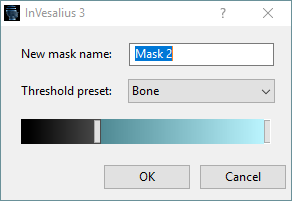
\includegraphics[scale=0.55]{segmentation_threshold_window_dialog_en.png}
\caption{Creating a new mask.}
\label{fig:create_new_mask}
\end{figure}

\newpage

After the segmentation it's possible to generate a corresponding 3D surface. The surface is formed by triangles. The following chapter will give more details about surfaces.

Click on the \textbf{Create surface} button (figure~\ref{fig:generate_surface}) to create a new surface. If there is a surface created previously you may overwrite it with the new one. To do this select the option \textbf{Overwrite last surface} before creating the new surface.

\begin{figure}[!htb]
\centering
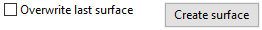
\includegraphics[scale=0.55]{segmentation_generate_surface_en.png}
\caption{Create surface button.}
\label{fig:generate_surface}
\end{figure}

After a few moments the surface will be displayed at the 3D visualization window of InVesalius (figure~\ref{fig:surface}).

\begin{figure}[!htb]
\centering
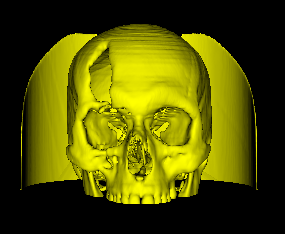
\includegraphics[scale=0.5]{surface_from_threshold.png}
\caption{3D surface.}
\label{fig:surface}
\end{figure}



\section{Manual segmentation (Image edition)}

Thresholding segmentation may not be efficient in some case since it's applied to the whole image. Manual segmentation may be used o segment only an isolated image region. Manual segmentation turns possible to add or remove some image regions to the segmentation. Manual segmentation requires more knowledge of  human anatomy. To use it click on \textbf{Manual edition} (figure~\ref{fig:advanced_edition}) to open the manual segmentation panel.

\begin{figure}[!htb]
\centering
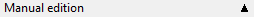
\includegraphics[scale=0.75]{segmentation_manual_label_en.png}
\caption{Icon to open the Manual segmentation panel.}
\label{fig:advanced_edition}
\end{figure}

Figure~\ref{fig:edition_slices_ref} show the Manual segmentation panel.

\begin{figure}[!htb]
\centering
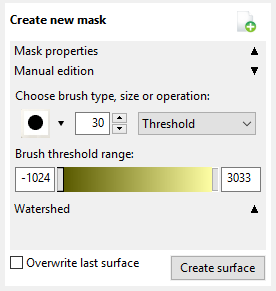
\includegraphics[scale=0.6]{segmentation_manual_window_en.png}
\caption{Manual segmentation panel.}
\label{fig:edition_slices_ref}
\end{figure}

There are two brushes used to segmentation: a circle and a square. Click on triangle icon (see figure~\ref{fig:brush_type}) to and click on the desired brush.

\begin{figure}[!htb]
\centering
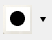
\includegraphics[scale=0.9]{segmentation_manual_pencil_type.png}
\caption{Brush types.}
\label{fig:brush_type}
\end{figure}

\newpage

It's also possible to adjust the brush size, like shown in the figure~\ref{fig:select_diameter}.

\begin{figure}[!htb]
\centering
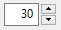
\includegraphics[scale=0.8]{segmentation_manual_diameter.png}
\caption{Adjusting the brush size.}
\label{fig:select_diameter}
\end{figure}

It's needed to select the operation to be performed by the brush. These are the options:

\textbf{Draw}: to add a non-selected region to the segmentation;

\textbf{Erase}: to remove a selected region from the segmentation;

\textbf{Threshold}: applies the thresholding locally, adding or removing a
region if in inside or outside of the threshold range.

Figure~\ref{fig:select_brush_operations} shows the operations.

\begin{figure}[!htb]
\centering
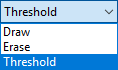
\includegraphics[scale=0.7]{segmentation_manual_pencil_type_operation_type_en.png}
\caption{Brush operations}
\label{fig:select_brush_operations}
\end{figure}

Figure~\ref{fig:noise_amalgaman} shows a image with noises caused by the presence of dental prosthesis. See the rays emerging from the dental arch. The thresholding segments the noise since its intensity is inside of the threshold of bone.

\begin{figure}[!htb]
\centering
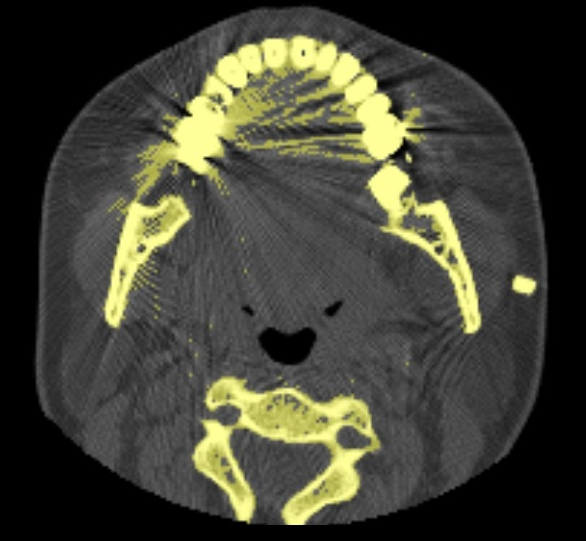
\includegraphics[scale=0.3]{segmentation_manual_noise_amalgam.jpg}
\caption{Noisy image segmented with threshold.}
\label{fig:noise_amalgaman}
\end{figure}

Figure~\ref{fig:surface_amagaman} shows a surface create from that segmentation.

\begin{figure}[!htb]
\centering
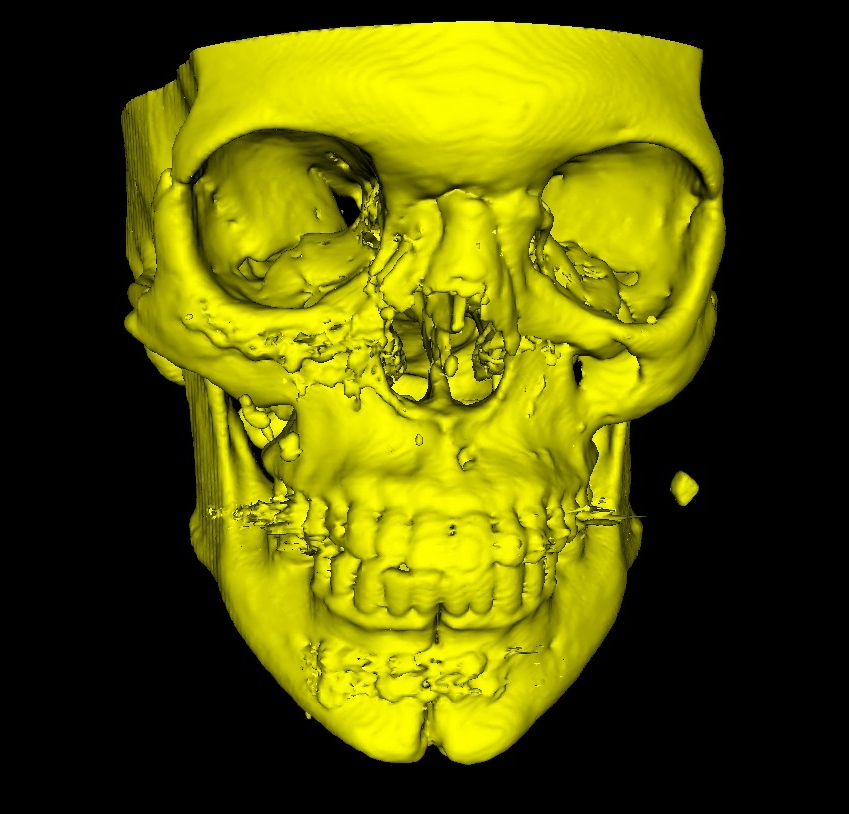
\includegraphics[scale=0.3]{segmentation_manual_noise_amalgam_3d.jpg}
\caption{Surface generated from noisy image.}
\label{fig:surface_amagaman}
\end{figure}

\begin{figure}[!htb]
\centering
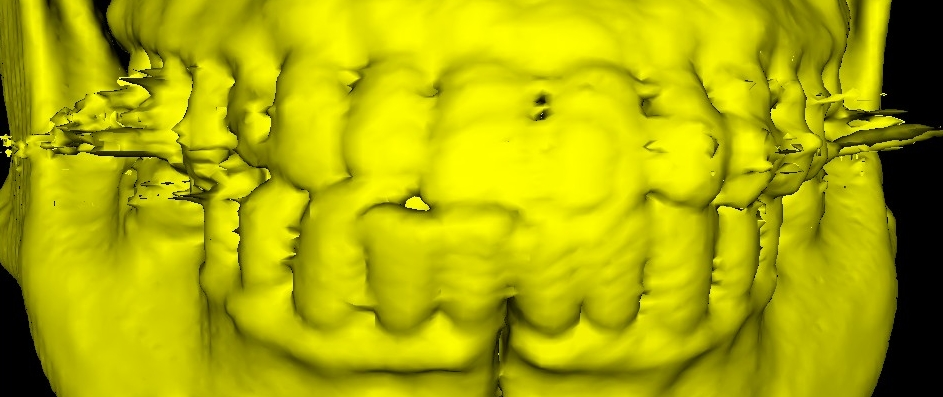
\includegraphics[scale=0.3]{segmentation_manual_noise_amalgam_3d_zoom.jpg}
\caption{Zoom in the noisy area.}
\label{fig:surface_amagaman_zoom}
\end{figure}

In such cases use the manual segmentation with the \textbf{erase} brush. Keep the \textbf{left} mouse button pressed while dragging the brush over region you want to remove (in mask).

Figure\ref{fig:editor_amalgaman} shows the image from figure~\ref{fig:noise_amalgaman} after the edition.

\begin{figure}[!htb]
\centering
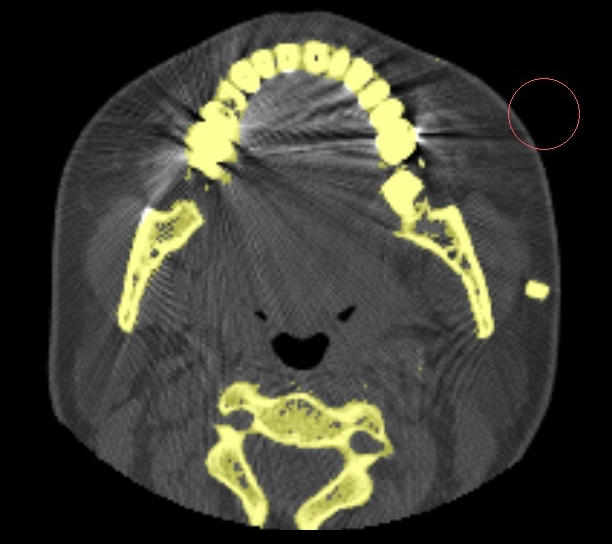
\includegraphics[scale=0.3]{segmentation_manual_noise_amalgam_removed.jpg}
\caption{After removing the noise.}
\label{fig:editor_amalgaman}
\end{figure}

\begin{figure}[!htb]
\centering
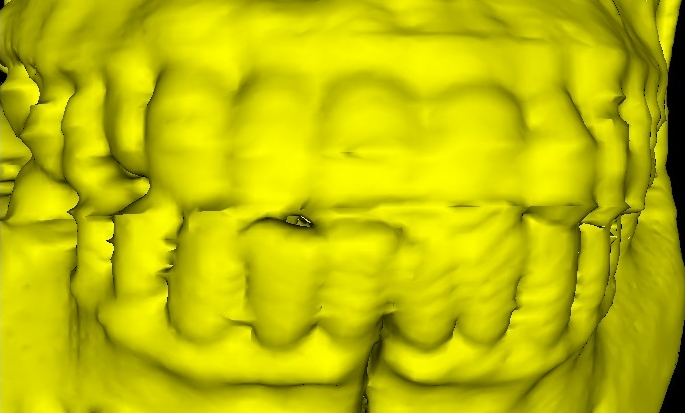
\includegraphics[scale=0.3]{segmentation_manual_noise_amalgam_removed_3d_zoom.jpg}
\caption{Surface generate after removing the noise.}
\label{fig:surface_edited_amalgaman}
\end{figure}

Realizada a edição, basta gerar a superfície a partir da imagem editada (figure \ref{fig:surface_edited_amalgaman}). Como houve edição, ao clicar em \textbf{Criar superfície}, será requerido se deseja gerar a superfície a partir do método \textbf{binário} ou utilizando o método de suavização \textbf{Suavização sensível ao contexto} (figure \ref{fig:new_surface_edited}) para minimizar os "degraus" na superfície.  Demais detalhes serão discutidos no capítulo \ref{cap_surface}.
%\ref{fig:generate_surface}).

It's possible to generate a surface after manual segmentation (figure~\ref{fig:surface_edited_amalgaman}). Since it was used the manual segmentation, when you click on \textbf{Create surface} button, a dialog (figure~\ref{fig:new_surface_edited}) will be opened to  to select if the surface will be created with the method \textbf{Binary} (blocky aspect) or \textbf{Context aware smoothing} (smoother).


\begin{figure}[!htb]
\centering
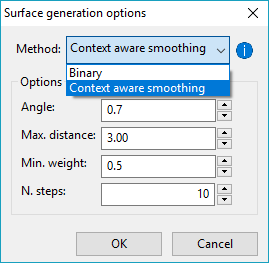
\includegraphics[scale=0.5]{surface_generation_dialog_en.png}
\caption{Surface creation methods}
\label{fig:new_surface_edited}
\end{figure}


\section{Watershed}

In watershed segmentation the user indicates with marks what is object and what is background. This method treats the image as watershed (hence the name watershed) in which the gray values (intensity) are the altitudes, forming valleys and mountains. The markers are water source. The waters fill the watershed until the waters gather together segmenting, this way, the background from the object. To use Watershed segmentation click on \textbf{Watershed} to open the watershed panel (figure~\ref{fig:watershed_painel}).

\begin{figure}[!htb]
\centering
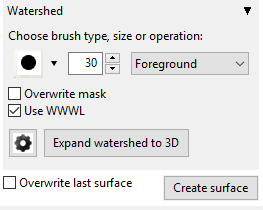
\includegraphics[scale=0.75]{segmentation_watershed_panel_en.png}
\caption{Watershed segmentation panel.}
\label{fig:watershed_painel}
\end{figure}

Before starting to segment with watershed it recommended to clean the mask (see section~\ref{cap:limpeza_mascara}).

To insert a marker (object or background) is used a brush, like when manual segmenting. You can use a circle or square brush and set its size.

It necessary to select the brush operation, which are the following:
\begin{itemize}
    \item \textbf{Object}: to insert object markers;
    \item \textbf{Background}: to insert background markers (not object);
    \item \textbf{Delete}: to delete markers;
\end{itemize}


The option \textbf{Overwrite mask} is used when the user wants that the result of watershed segmentation overwrites the existent segmentation. The option \textbf{Use WWWL} is used to make watershed take into account the image with the values of \textbf{window width} and \textbf{window level} not the raw one, which may result in better segmentation.

Click on the button on the left side of the panel (figure~\ref{fig:watershed_conf}) to access more watershed configurations. This button will open a dialog (figure~\ref{fig:watershed_janela_conf}). The method option allows to choose the Watershed algorithm to be used to segment. It may be the conventional \textbf{Watershed} or \textbf{Watershed IFT}, which is based on the IFT (\textit{Image Forest Transform}) method. In some cases, like brain segmentation, the \textbf{Watershed IFT} may have a better result.

The connectivity option refers to the pixel neighbourhood which may be $4$ or $8$ when in 2D,  or $6$, $18$ or $26$ when in 3D. \textbf{Gaussian sigma} is a parameter used in the smoothing algorithm (the image is smoothed before the segmentation to remove the noise and get better results). The greater this value the smoother the smoother the image will be.

\begin{figure}[!htb]
    \centering
    
\includegraphics[scale=0.5]{configuration.png}
    \caption{Button to open the Watershed configuration dialog.}
    \label{fig:watershed_conf}
\end{figure}

\begin{figure}[!htb]
    \centering
    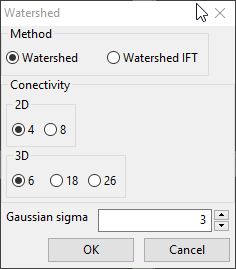
\includegraphics[scale=0.55]{segmentation_watershed_conf_en.png}
    \caption{Watershed configuration dialog.}
    \label{fig:watershed_janela_conf}
\end{figure}

Normally, the \textbf{Watershed} is applied only in one slice, not in the whole image. After adding the markers is possible to apply the watershed to the whole image, just click on the button \textbf{Expand watershed to 3D}. Figure~\ref{fig:watershed_2d} shows the result of watershed segmentation in a slice (2D) of brain image. Figure~\ref{fig:watershed_3d} shows the segmentation expanded to the whole image (3D).

Figure~\ref{fig:watershed_2d} also shows the object markers (in light green), the background markers (in red) and the segmentation mask (in green) overlaying the selected regions (result).

\begin{figure}[!htb]
\centering
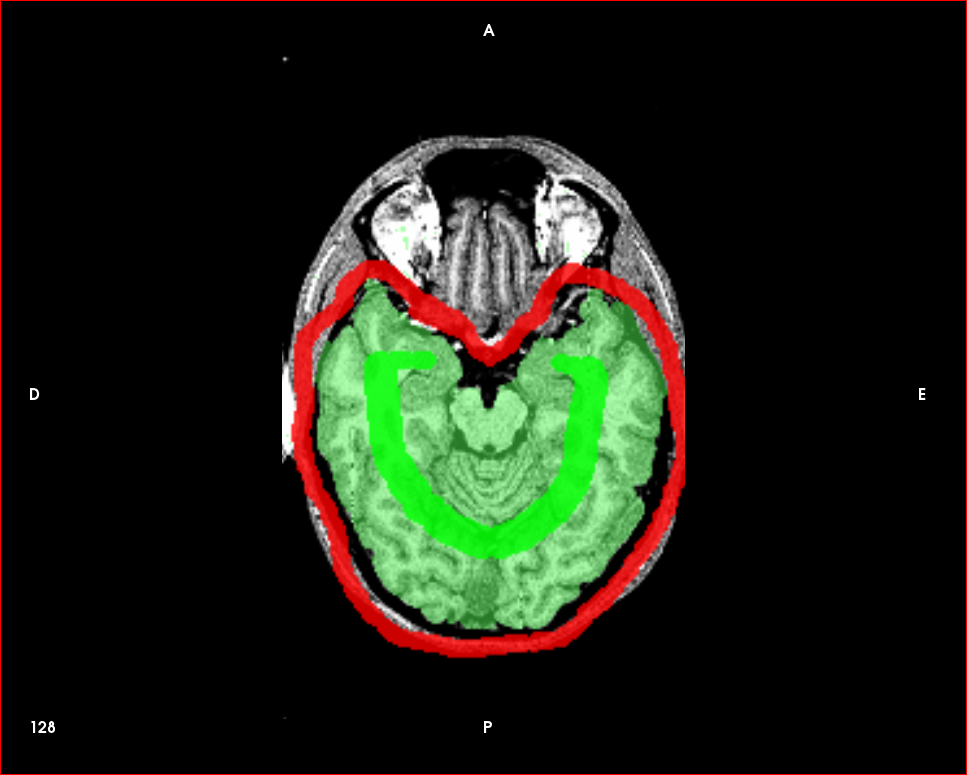
\includegraphics[scale=0.2]{segmentation_watershed_axial.png}
\caption{Watershed applied to a slice.}
\label{fig:watershed_2d}
\end{figure}

\begin{figure}[!htb]
\centering
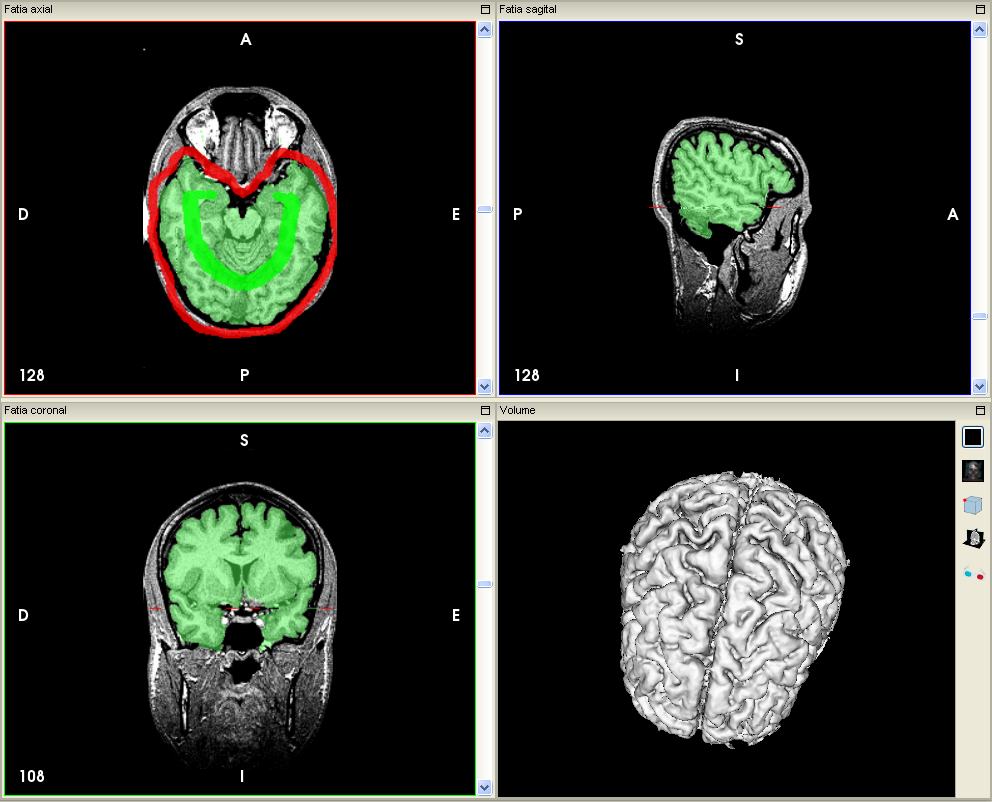
\includegraphics[scale=0.4]{segmentation_watershed_multiplanar_3d_pt.png}
\caption{Brain segmentation using the watershed method applied to the whole image (3D).}
\label{fig:watershed_3d}
\end{figure}

\section{Region growing}

Region growing tool is accessed in the menu \textbf{Tools}, \textbf{Segmentation}, \textbf{Region growing} (figure~\ref{fig:menu_segmentation_region_growing}). Before segmenting select if the operation will be in \textbf{2D - Actual slice} or \textbf{3D - All slices}. It is also necessary to select the connectivity: $4$ or $8$ to 2D or $6$, $18$ or $26$ to 3D. It's also necessary to select the method, which may be \textbf{Dynamic, Threshold, or Confidence} (figure~\ref{fig:segmentation_region_growing_dinamic})

\begin{figure}[!htb]
    \centering
    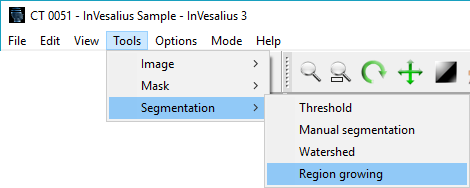
\includegraphics[scale=0.5]{menu_segmentation_region_growing_en.png}
    \caption{Menu to access the region growing segmentation segmentation tool.}
    \label{fig:menu_segmentation_region_growing}
\end{figure}

\begin{figure}[!htb]
    \centering
    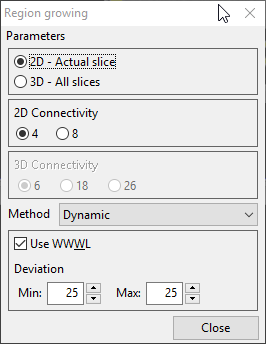
\includegraphics[scale=0.7]{segmentation_region_growing_dinamic_en.png}
    \caption{Dialog to configure the parameters of region growing segmentation tool.}
    \label{fig:segmentation_region_growing_dinamic}
\end{figure}

A técnica parte de um pixel inicial que é indicado clicando com o \textbf{botão direito} do mouse, os pixels vizinhos que satisfazem as condições indicadas anteriormente são selecionados. Cada método leva em consideração diferentes condições, a seguir são apresentadas as diferenças entre cada método:

This segmentation technique starts with a pixel (indicated by the user clicking with the left-button of the mouse). If the neighbour pixels meet some conditions are selected. Iteratively, the selection expands analyzing the neighbourhood of the selected pixels. Each region growing method has a different condition of selection:

\begin{itemize}
	\item \textbf{Dynamic}: In this method uses the value of the pixel clicked by the user. Then every connected pixel inside the lower (min) and the upper (max) range deviation are selected. The option \textbf{Use WWWL} is default and makes region growing taking into account the image with \textbf{window width} and \textbf{window level} applied not the raw one (figure~\ref{fig:segmentation_region_growing_dinamic_parameter}).

	\begin{figure}[!htb]
	\centering
	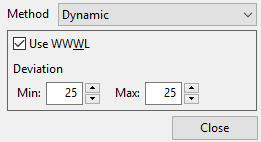
\includegraphics[scale=0.7]{segmentation_region_growing_dinamic_parameter_en.png}
	\caption{Dynamic method parameters.}
	\label{fig:segmentation_region_growing_dinamic_parameter}
	\end{figure}

	\item \textbf{Threshold}: This method selects the pixels whose intensity are inside the minimum and maximum threshold (figure~\ref{fig:segmentation_region_growing_limiar}).

	\begin{figure}[!htb]
	\centering
	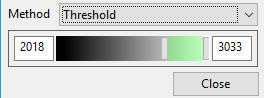
\includegraphics[scale=0.7]{segmentation_region_growing_limiar_en.png}
    \caption{Adjust the threshold.}
	\label{fig:segmentation_region_growing_limiar}
	\end{figure}

    \item \textbf{Confidence}: This method starts by calculating the standard deviation and the mean value of the pixel selected by the user and its neighbourhood. Connected pixels with value inside the range (given by the mean more and less the standard deviation multiplied by the \textbf{Multiplier} parameter). It's calculated the mean and the standard deviation from the selected pixels. Which follows by other expansion step. This process is repeated according to the number of \textbf{Iterations} parameter. The figure~\ref{fig:segmentation_region_growing_confidence_parameter} shows the parameters for this method.

	\begin{figure}[!htb]
	\centering
	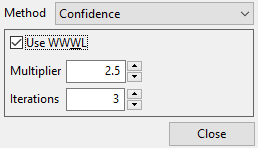
\includegraphics[scale=0.7]{segmentation_region_growing_confidence_parameter_en.png}
    \caption{Confidence parameter.}
	\label{fig:segmentation_region_growing_confidence_parameter}
	\end{figure}


\end{itemize}
